\documentclass[10pt,a4paper,onecolumn]{article}
\usepackage[latin1]{inputenc}
\usepackage{amsmath}
\usepackage{amsfonts}
\usepackage{amssymb}
\usepackage{listings}
\usepackage{graphicx}
\usepackage{epstopdf}

\lstset{language=Haskell}
\lstset{breaklines=true}
\author{Beerend Lauwers \and Frank Wijmans}
\title{Static-link optimisation: Documentation}
\date{\today}
\begin{document}
	\maketitle
	
	\section{Introduction}
    
    This document describes the workings of our static-link optimisation implementation.

	\section {Overview}
    
    Our optimization does the following steps:
    \begin{enumerate}
        \item Synthesize all used variables in a function declaration and collect it in the $ usedvars $ attribute.
        \item For each used variable, calculate its depth. Local variable = 0, one scope higher = 1, etc. Collect this information in a tuple of $(Ident,Int)$.
        \item Sort this list of tuples by depth, and then pass it down to $ Exp $ level again.
        \item Pass the synthesized $ env $ attribute down to the $ Exp $ level (local variables only). This way, the correct offsets for static-link paths can be calculated.
        
        \begin{figure}[htb]
        \centering
        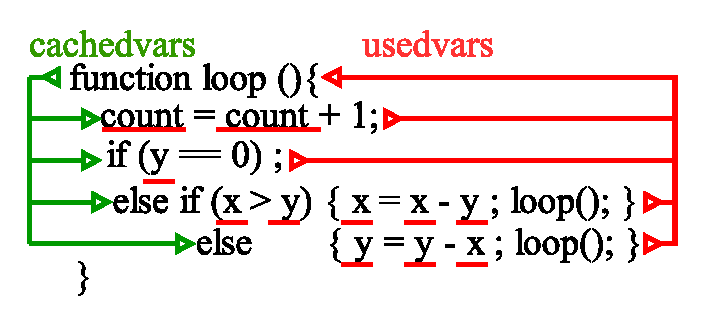
\includegraphics{tofrom.eps}
        \caption{Using two passes to get the necessary info to the correct levels. The same process occurs for $ env $ and $ localvars $.}
        \end{figure}

        \item The following optimizations are done during code generation:
        \begin{description}
            \item[FunDecl] Cache static-link paths of variables whose depth is larger than one. (Caching depths smaller than two results in an increase of code instead of a decrease.)
            \item[Assign and Var] Using the $ get' $ and $ set' $ functions, check if a variable's static-link path is cached. If so, use the static-link path. Otherwise, use the original $ get $ / $ set $ function.
            \item[FunDecl and Return] In the $ return\_ $ function, take into account the extra size used up by cached static-link paths.
        \end{description} 
    \end{enumerate}
    
    \section {Implementation details}
    
    \subsection {Generating $ cachedvars $}
	First, we get rid of local variables and double variables by doing
	\begin{lstlisting}
nub @b.usedvars \\ (map fst $ @b.env)
	\end{lstlisting} 
	Then, we are ready to generate the depth of the variables. 
	Each variable's depth is calculated by traversing the symbol table. Every time we go deeper into the symbol table, we increase our depth by 1.
	Finally, we sort our list of tuples by depth. This way, we can use the implicit ordering of the list to get the correct cached static-link path for a certain depth.

    \subsection {Creating cache code}
	Our $ cache $ function is relatively simple: it takes an offset (the amount of local variables in the function's declaration), the $ cachedvars $ list, and the symbol table.
	First, it removes function parameters and variables that are accessible at one scoper higher: caching these results in less efficient code.
	It then reduces the pruned $ cachedvars $ list even more to only have a single variable for every depth in the list:
	\begin{lstlisting}
[("x",2),("y",2),("count",3)]
	\end{lstlisting} 
	becomes
	\begin{lstlisting}
[("y",2),("count",3)] 
	\end{lstlisting} 
	This list is mapped over with $ cacheAddress $, which generates code to store the static-link path.

    \subsection {Setting and getting global variables}
	We introduced two new functions for setting and getting, namely $ set' $ and $ get' $.
	These functions also receive an offset, the variable name, the symbol table and the list of cached variables.
	The function checks if a variable is in the list of cached variables, and, if so, fetches the offset to the cached static-link path. Otherwise, it uses the original function to generate the appropriate code.

    \subsection {Updating the $ return\_ $ function}
	The $ return\_ $ function has to be updated as well: adjusting the stack pointer must now also take into account the cached static-link paths.
	Hence, the function takes the $ cachedvars $ list, does the same removals as the $ cache $ function, and gets the $ length $ of the resulting list.

    
\end{document}